\documentclass[a4paper, 12pt]{report}


\usepackage[utf8]{inputenc}
\usepackage[T1]{fontenc}
\usepackage[spanish]{babel} 
\usepackage{graphicx}
\usepackage{amsmath}
\usepackage{amssymb}
\usepackage{mathtools}
\usepackage{amsthm}
\usepackage{bbm}
%\usepackage[shortlabels]{enumitem}
\usepackage{enumerate}
\usepackage{array,tabularx}
\usepackage{float}
\usepackage{wrapfig}
\usepackage[export]{adjustbox}
\usepackage[rightcaption]{sidecap}
\usepackage{multirow}
\usepackage{subfig}
\usepackage{capt-of}
\usepackage{captdef}
\usepackage{color}
\usepackage{ebproof}
\usepackage{soul}
\usepackage{hyperref}
\usepackage{ebproof}
\usepackage{stmaryrd}
\usepackage{fullpage}
\usepackage{xcolor}

\newcommand{\Ra}{\Rightarrow}
\newcommand{\ra}{\rightarrow}
\newcommand{\N}{\mathbb{N}}
\newcommand{\R}{\mathbb{R}}
\newcommand{\te}{\text}
\newcommand{\Lra}{\Leftrightarrow}
\newcommand{\lra}{\leftrightarrow}

\begin{document}

\centerline{\Huge\bf Apuntes de Introducción a la Computación}



\tableofcontents

\chapter{Introducción}

 En este curso planteo a grandes rasgos tres objetivos. El primero es que aprendan las bases de la programación. 
Otro objetivo es que desarrollen la capacidad de utilizar las computadoras con fines matemáticos, como por ejemplo para determinar si un número es primo, o aproximar numéricamente el valor de una integral, o generar gráficas de distintos tipos.
El otro objetivo es que desarrollen la capacidad de entender la computación como un concepto abstracto matemático, para desarrollar programas en base a razonamiento matemático y además poder demostrar matemáticamente propiedades sobre estos programas.
De modo sintético, este curso se trata de programación, de computación para matemática y de matemática para computación.

Se espera que los contenidos de este capítulo aporten intuiciones que ayuden a comprender la materia.



\section{Conceptos básicos de computación e intuiciones}

La computación se trata de operaciones definidas por reglas precisas que operan con objetos finitos y en una cantidad finita de pasos llegan a un resultado.

Los objetos finitos, a los que en general llamaremos {\bf datos}, pueden ser por ejemplo números naturales, palabras o listas finitas. Cabe aclarar que al decir que los números naturales son finitos nos referimos a que cada número natural es un objeto finito. Por supuesto que el conjunto de todos los números naturales, por otra parte, es infinito.

A una operación definida por reglas precisas que opera con datos y termina en finitos pasos le llamaremos {\bf algoritmo}. Un programa es lo mismo que un algoritmo. Un ejemplo de algoritmo es el de la suma que se aprende en la escuela. Dados dos números, aplicando una secuencia finita de pasos bien definida se llega al resultado.


Una buena analogía consta de las recetas de cocina. Sin embargo, hay una diferencia importante. En las recetas de cocina, por la naturaleza de la situación, pueden haber ciertas ambigüedades, o puntos en los que hay que tomar una decisión, de modo que si dos personas realizan la misma receta el resultado puede ser distinto, sin que ninguno de los dos lo haya hecho mal. Pueden haber frases como <<un poquito de sal>> que según la persona se traduzcan a distintas cantidades. En computación, un algoritmo bien ejecutado debe tener un único resultado correcto, como ocurre con la suma. Que las reglas sean precisas significa que no hay margen de variabilidad en lo que se debe hacer, ni puntos en los que un ser con voluntad propia deba pensar y tomar una decisión. Esto es importante por dos motivos. Primero, asegura que si se realiza por una persona, hay un único resultado correcto. Segundo (y tal vez más importante), es necesario para que pueda ser realizado automáticamente por una computadora, que en lugar de un ser con pensamiento y voluntad es una cosa.

Como los algoritmos deben estar bien definidos y no puede haber ninguna ambigüedad, son en esencia conceptos matemáticos. De hecho, la computación teórica es una rama de la matemática.
\subsection{Bases de la formalización matemática}

Una forma de representar algoritmos en computación teórica es mediante funciones $f:\N\to\N$, donde la idea es que si $n$ es la entrada del programa, entonces $f(n)$ es la salida. Como se trata de un algoritmo, no puede ser cualquier función, sino una que puede calcularse en finitos pasos con reglas precisas. A primera vista puede parecer que usar solamente números naturales es una restricción, pero de hecho alcanza para hablar de todo lo que se puede programar. De hecho, dentro de la computadora todos los distintos tipos de datos  se representan con secuencias de bits (\emph{binary digits}, es decir dígitos binarios: 0 o 1) y cualquier secuencia de bits se puede interpretar también como un número escrito en binario. Por lo tanto, todos los datos finitos se pueden representar con números (en general muy grandes). Debido a esto, un programa que recibe como entrada una imagen y retorna la imagen con alguna modificación, por ejemplo, se puede ver como una función $f:\N\to\N$ que recibe el número que codifica la imagen original y retorna el número que codifica la imagen modificada.

Hay distintos formalismos que permiten definir funciones $f:\N\to\N$ computables, es decir, que corresponden a algoritmos. Algunos de ellos son las máquinas de Turing, el cálculo lambda y la teoría de las funciones recursivas. Notablemente, aunque todos son formalismos muy distintos, siempre dan lugar a exactamente el mismo conjunto de funciones computables. Este conjunto de funciones computables no es todo $\N^\N$. De hecho, el conjunto de las funciones computables es numerable, por lo que la mayoría de las funciones no lo son.

Por último, está la pregunta de si la definición matemática de función computable corresponde con las funciones que en el mundo físico se pueden calcular con una computadora. La Tesis de Church-Turing conjetura que efectivamente es el caso. Al ser algo del mundo físico y salirse de la matemática, no hay ninguna prueba formal, pero en general es asumido como cierto.


\section{Arquitectura de Von Neumann}\label{sec-ArqVonNeu}

La arquitectura de Von Neumann es un modelo para computadoras físicas, a diferencia de formalismos como las máquinas de Turing, que son conceptos puramente teóricos.

Primero sería bueno decidir qué consideramos como una computadora. Digamos que es un dispositivo físico que puede automáticamente calcular funciones computables y que tiene mecanismos para interactuar con el entorno. Podemos pensar que es una caja negra que de alguna forma calcula funciones computables y además tiene algún mecanismo por el cual podemos ingresar información (por ejemplo con un teclado) y algún mecanismo por el cual puede devolver información (por ejemplo con una pantalla).

La arquitectura de Von Neumann define que la computadora tiene tres componentes principales que interactúan entre sí: un {\bf procesador }(CPU), una {\bf memoria} y un subsistema de {\bf entrada y salida} (figura \ref{fig-ArqVN}). A la conexión entre las distintas componentes se le llama {\bf bus}. El procesador es un dispositivo con la capacidad de ejecutar un conjunto finito de operaciones básicas, llamadas  instrucciones. La idea es que un programa está dado por una secuencia finita de instrucciones. Si bien las instrucciones son finitas (y en general bastante sencillas), al usarlas de forma secuencial se puede implementar cualquier función computable. Tanto la secuencia de instrucciones que conforma un programa como los datos con los que este opera se guardan en la memoria. El subsistema de entrada y salida permite que la computadora interactúe con el entorno (por ejemplo con un usuario que ingresa datos y observa resultados o con otra computadora dentro de una red).

Todas las componentes de la computadora se construyen con circuitos electrónicos y usando la abstracción del {\sl bit}, que significa dígito binario, es decir {\tt 0} o {\tt 1}. Claramente el bit es un concepto abstracto que no existe de por sí en los circuitos eléctricos. Lo que se hace es tomar una convención, como que si circula corriente significa 1 y si no significa 0, o que cierto voltaje significa 1 y cierto voltaje significa 0. Sea cual sea la convención, lo importante es que se pueden construir circuitos con entrada y salida que implementen cualquier operación finita. Por ejemplo, se puede armar un circuito con 4 bits de entrada, $a_0,a_1,b_0,b_1$ y tres bits de salida $c_0,c_1,c_2$ tal que si tomamos la entrada como la codificación en binario de dos números entre $0$ y $3$, la salida sea la codificación en binario de la suma. En general, para cada función $f:\{0,1\}^n\to\{0,1\}^m$ se puede construir un circuito con $n$ bits de entrada y $m$ bits de salida que implementa la función~$f$. A estos se les llama {\sl circuitos combinatorios}. Junto con otro tipo de circuitos llamados {\sl secuenciales} (que funcionan por etapas y además de la entrada actual dependen de las entradas anteriores, o de un estado que puede ir variando), son un elemento base de las computadoras, tal vez el principal.




\begin{figure}
	\centering
	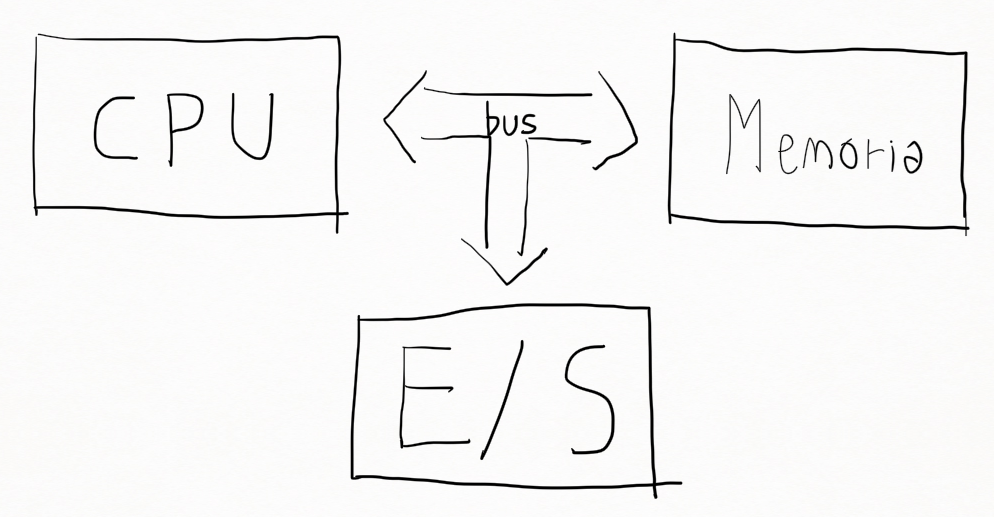
\includegraphics[scale=0.3]{ArqVN.png}
	\caption{Esquema de los componentes de la arquitectura de Von Neumann}
	\label{fig-ArqVN}
\end{figure}

El procesador tiene tres componentes que cumplen distintas funciones: la unidad de control, la unidad aritmética lógica (ALU) y el banco de registros. La unidad aritmética lógica consta de varios circuitos combinatorios que implementan operaciones básicas, como por ejemplo operaciones lógicas como <<y>>, <<o>> y <<no>>, operaciones aritméticas como suma y multiplicación (para números codificado con una cantidad fija de bits) u operaciones básicas sobre cadenas e bits, como el {\sl shift}, que traslada cada bit un lugar a la derecha o la izquierda. El banco de registros consta de ciertos registros (un tipo de circuito que almacena valores) en general variables que se usan para el funcionamiento de la CPU. Por ejemplo, pueden tener los argumentos de las operaciones que va a realizar la unidad aritmética lógica. También hay un registro de particular importancia llamado {\sl program counter}, que indica la posición de memoria de la siguiente instrucción a ejecutar (es de suma importancia, ya que la idea del CPU es ejecutar secuencias de instrucciones). Finalmente, la unidad de control es un circuito secuencial que se encarga de llevar a cabo las instrucciones, usando la unidad aritmética lógica y el banco de registros. Estos circuitos secuenciales están hechos para que automáticamente se lea e identifique la instrucción que indica el program counter, se carguen nuevos datos en los registros (si es necesario), se realice la operación indicada en la ALU y se guarde el resultado donde corresponda (si hay que hacer alguna operación), y que el program counter avance a la siguiente instrucción, para poder repetir el proceso.

Respecto a la suma, la ALU al ser un circuito combinatorio, es en realidad como una tabla que tiene el resultado para cada combinación de operandos. Las sumas que se realizan directamente por la ALU pueden ser por ejemplo de números representados por uno o dos bytes (donde un byte es por definición una secuencia de 8 bits). Como la cantidad de números representables crece exponencialmente con la cantidad de bits, hacer sumas de números más grandes por la ALU (que lo que hace es tener una tabla con todos los resultados) es extremadamente ineficiente. Lo que se hace para realizar sumas con números más grandes es descomponerlas como una secuencia de instrucciones más sencillas. Esto es como lo que se hace en los algoritmos aritméticos básicos. Pensemos por ejemplo en el producto. Está la tabla de multiplicación que uno se aprende de memoria (lo cual es análogo a lo que está en los circuitos de la ALU) pero luego a partir de eso, siguiendo un algoritmo (secuencia de instrucciones) se puede calcular la multiplicación de números de cualquier cantidad de cifras sin precisar saber nada más de memoria.

Algunos ejemplos de instrucciones comunes son...

La memoria...

La figura ... es un esquema de una computadora un poco más elaborado.






\end{document}


